
\begin{multicols}{2}
La figure ci-contre représente une pyramide
régulière $SABCD$ à base carrée, de sommet $S$, de hauteur
$SH$. L'unité est le centimètre et on a $SH=6$ et $AD=8$.\\
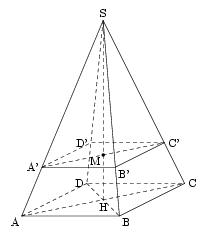
\includegraphics[scale=1]{RepS-45.png} 
\end{multicols}

\begin{enumerate}
\item Calcule le volume de la pyramide $SABCD$.
\item On appelle $M$ le point du segment $[SH]$ tel que
$SM=\dfrac34SH$. On coupe la pyramide $SABCD$ par un plan
parallèle à la base et passant par $M$, comme indiqué sur la figure.
\begin{enumerate}
\item Quelle est la forme du quadrilatère $A'B'C'D'$ ?
\item Calcule le volume de la pyramide $SA'B'C'D'$.
\end{enumerate} 
\end{enumerate}

